\chapter{Nuova architettura}
\label{cha:nuova_architettura}

In seguito alla scelta del framework da utilizzare, i due passaggi successivi per
iniziare ad utilizzare il nuovo sistema sono: creare una nuova infrastruttura (macchina
virtuale dedicata) per Airflow, portare la vecchia implementazione sulla nuova infrastruttura
e scegliere una strategia per il rilascio in produzione. Nelle sezioni seguenti
verranno discusse dettagliatamente le fasi di migrazione e alcune decisioni
implementative.

\begin{figure}[htbp]
  \centering
  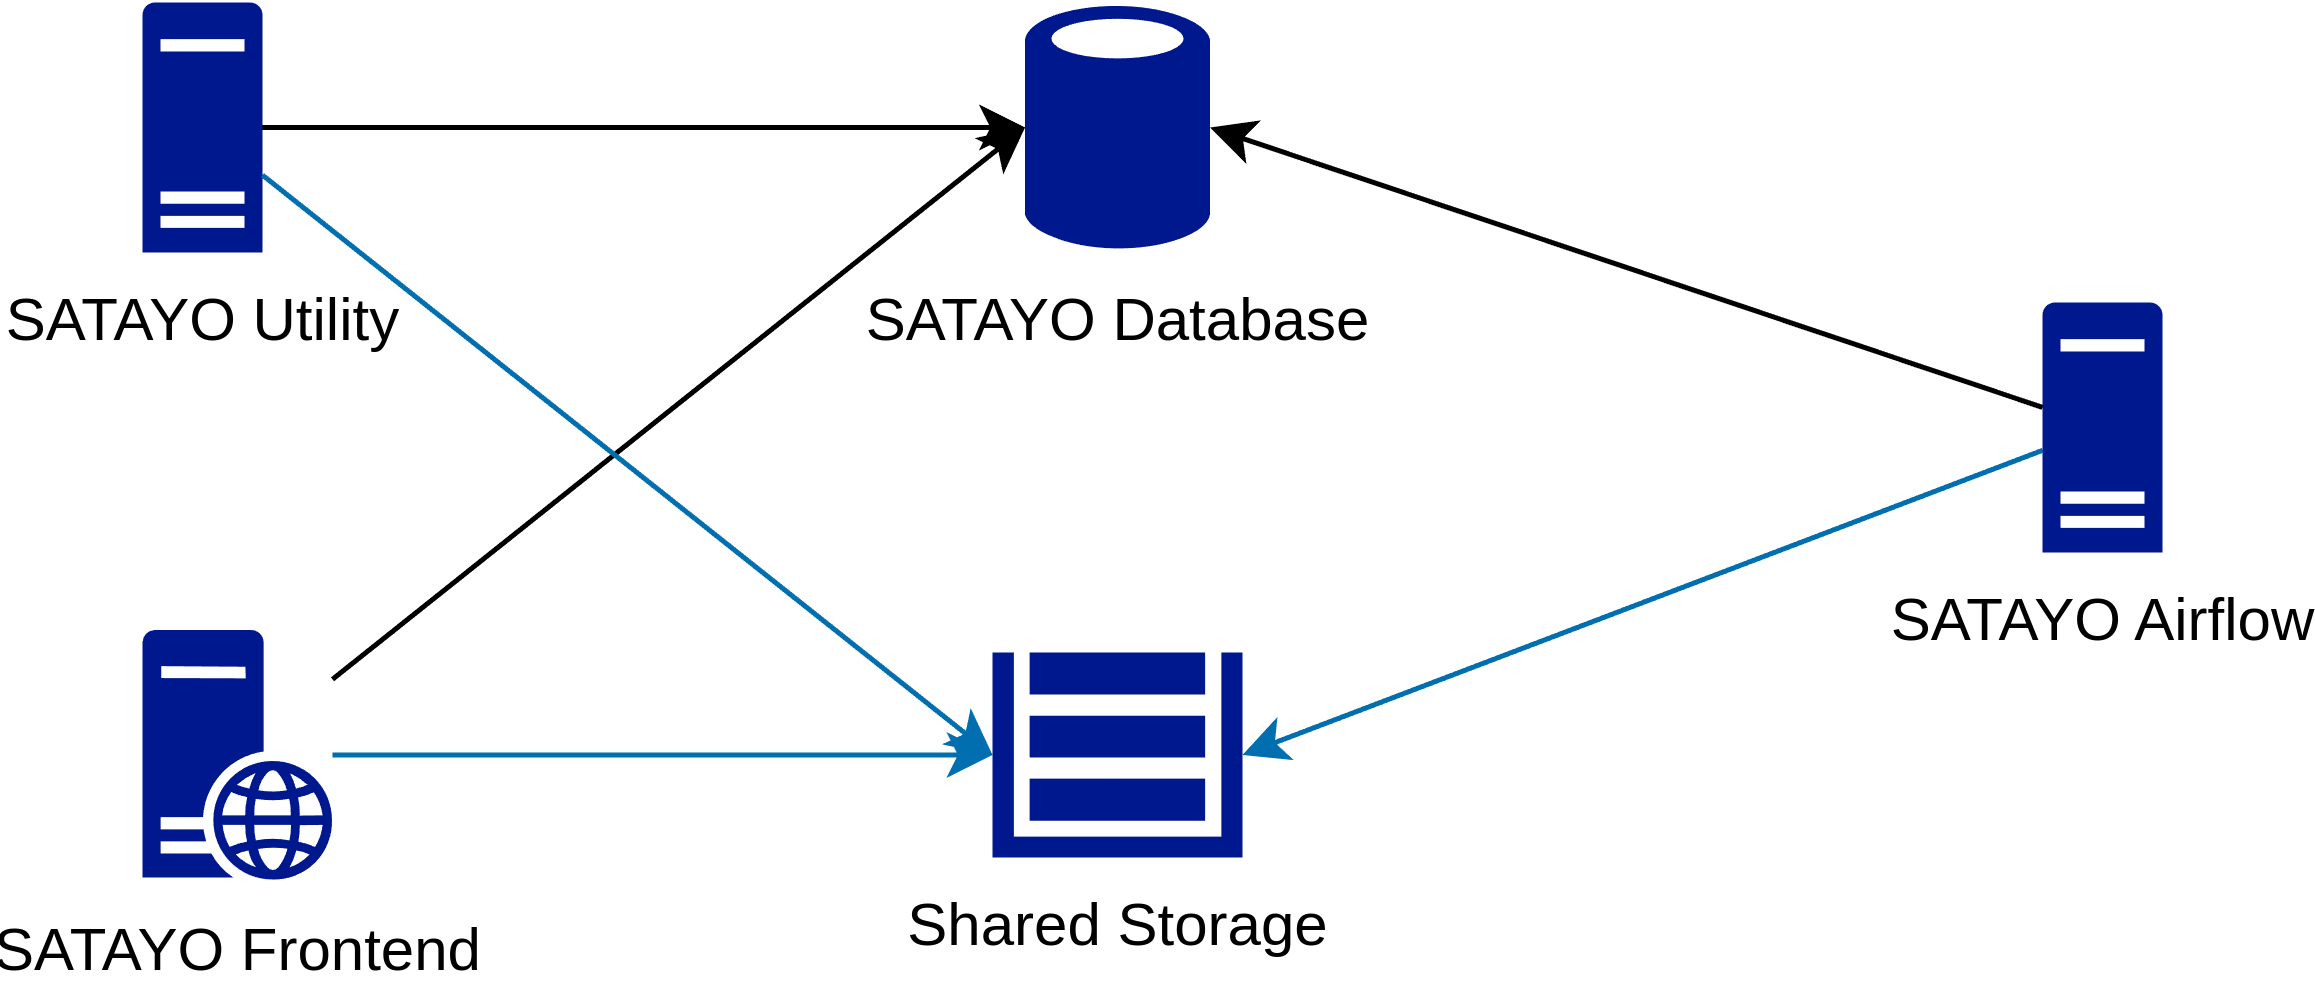
\includegraphics[width=.6\linewidth]{images/SATAYO_infrastructure_new.png}
  \caption{Nuova infrastruttura di SATAYO}
  \label{fig:infra_new}
\end{figure}

\section{Implementazione e Containerizzazione}
\label{sec:impl_container}

Dopo una prima analisi dei metodi di deployment messi a disposizione da Airflow,
è stato deciso di procedere inizialmente con l'utilizzo di un'immagine Docker\cite{docker}
istanziata su più container gestiti tramite Docker Compose. Nonostante questo approccio
sia sconsigliato dalla documentazione, che incita ad usare Kubernetes per gli
ambienti di produzione, è stato il modo più veloce per ottenere un'ambiente funzionante.
Sebbene questa decisione possa sembrare, in primo luogo, che porterà ad
ulteriore debito tecnico, non è assolutamente il caso. Il \texttt{Dockerfile} che
è stato scritto per questa implementazione, infatti, può essere utilizzato anche
per il deployment su Kubernetes.

Il \texttt{Dockerfile} descrivente l'immagine utilizzata, è stato implementato utilizzando
come base l'immagine ufficiale di Airflow \texttt{apache/airflow} e aggiungendo
tutte le dipendenze e tool OSINT utilizzati dalle fasi di SATAYO. Questo ha permesso
di semplificare l'implementazione delle fasi, in quanto non deve più essere
eseguito un controllo a tempo di esecuzione per verificare la presenza del tool
da eseguire. Le altre modifiche effettuate sul codice della vecchia implementazione
delle task, consultabile in \ref{lst:task-impl-old}, sono state: rimuovere il
controllo sul \texttt{id\_tool\_progress}, in quanto su Airflow l'esecuzione
della task avviene soltanto dopo che le sue dipendenze sono state risolte, non necessitando
quindi di controlli secondari all'interno della funzione stessa; aggiungere il
decoratore \texttt{@satayo\_task} all'inizio della definizione di ogni fase, il
quale ha la funzione di provvedere gli argomenti in modo tale che la nuova
implementazione sia compatibile con quella vecchia. Queste modifiche si possono osservare
nel codice nuovo \ref{lst:task-impl-new}, in cui viene direttamente eseguito il
corpo della fase.

Come precedentemente riportato, attualmente Airflow è utilizzato tramite Docker Compose,
è quindi in funzione su una macchina singola e l'infrastruttura è come riportato
in figura \ref{fig:infra_new}.

\pagebreak
\lstinputlisting[language=Python, caption=Esempio di vecchia implementazione di una
fase di SATAYO, label=lst:task-impl-old]{listings/task-old.py}

\lstinputlisting[language=Python, caption=Esempio della nuova implementazione della
medesima fase, label=lst:task-impl-new]{listings/task-new.py}

\section{Retrocompatibilità}
\label{sec:retrocompatibility}

Per permettere una corretta integrazione del nuovo sistema all'interno di quello
corrente, mantenendo tutte le funzionalità presenti, è necessario continuare ad utilizzare
alcune funzionalità che potrebbero essere deprecate e sostituite interamente da Airflow.
In particolare occorre mantenere l'uso del \texttt{tool\_progress}, descritto
nella sezione \ref{sub:db:tasks}, in quanto esso viene utilizzato per calcolare la
data di ultima esecuzione di una determinata fase di SATAYO e per individuare la
fase che ha recuperato una certa evidenza. Per evitare la duplicazione di codice
è stato deciso di implementare questa funzionalità all'interno del decoratore
\texttt{@satayo\_task} (scritto utilizzando una classe Python) tramite le due funzioni
\texttt{pre\_task} e \texttt{post\_task}. L'implementazione dettagliata è
riportata in \ref{lst:retro}, si può notare come, nella prima funzione, eseguita
prima dell'esecuzione della task, venga utilizzato un \texttt{host\_id} dedicato
per le esecuzioni su Airflow, e sia creato un \texttt{tool\_progress} che riporta
le informazioni dell'esecuzione delle task come se venissero eseguite sul sistema
precedente. Nella seconda funzione, eseguita successivamente alla task, viene
invece impostata la data e lo stato di termine di essa. Per il caso di errore di
esecuzione viene chiamata una funzione di callback, presente tra gli argomenti
della task Airflow, che imposta il \texttt{tool\_progress} in stato di errore.

Un'altra funzionalità riportata momentaneamente è la possibilità di salvare
certi messaggi di log all'interno del database. Questo è stato fatto per avere visibilità
su certi errori che non terminerebbero con errore la task, ma sarebbe comunque
opportuno controllare in caso si presentassero.

\lstinputlisting[language=Python, caption={Implementazione delle funzioni di \texttt{@satayo\_task} che permettono la retrocompatibilità},
label=lst:retro]{listings/retrocompatibility-funcs.py}

\section{Ricerche schedulate}
\label{sec:schedulate}

Una delle funzionalità più interessanti di SATAYO per un cliente, è il monitoraggio
continuo della propria esposizione online. Per ottenere questo risultato è
essenziale eseguire determinate fasi secondo una schedulazione predefinita, nel dettaglio
ci saranno delle task che devono essere eseguite giornalmente, settimanalmente o
ogni due settimane. Ciò è implementato dalle seguenti operazioni: viene eseguita
una query per collezionare la lista di domini da monitorare; da questa lista vengono
generati dinamicamente 3 DAG per ogni dominio, ognuno di essi contenente le task
da eseguire rispettivamente ogni giorno, settimana o due settimane. Per
distribuire equamente nel tempo le esecuzioni dei DAG settimanali e
bisettimanali viene utilizzata la funzione riportata in \ref{lst:schedule}. Il funzionamento
di quest'ultima si basa sul fatto che un PRNG (PseudoRandom Number Generator)\cite{py-random},
inizializzato con lo stesso \texttt{seed}, produrrà la medesima sequenza di numeri.
Utilizzando quindi come \texttt{seed} il dominio da analizzare, i DAG riferiti
ad esso verranno eseguiti con intervalli regolari e in giorni costanti. Per i DAG
settimanali verrà scelto un giorno casuale della settimana, mentre per quelli
bisettimanali verranno casualmente scelti due giorni del mese distanti 14 giorni.

\lstinputlisting[language=Python, caption={Funzione che calcola una schedulazione pseudo randomica per ogni dominio},
label=lst:schedule]{listings/schedule-generation.py}

\section{Nuove ricerche}
\label{sec:nuove}

\lipsum[1]

\section{Task di sistema}
\label{sec:sistema}

\lipsum[1]

\section{Strategia di rilascio in produzione}
\label{sec:deployment}

\lipsum[1]

\section{Monitoraggio}
\label{sec:monitoraggio}

\lipsum[1]